\documentclass[hyperref={pdfpagelabels=false}]{beamer}
%\usepackage{href}
\usepackage{listings}
\usepackage[utf8]{inputenc}
\setbeamertemplate{section in toc}[sections numbered]
\setbeamertemplate{subsection in toc}[subsections numbered]
\newcommand{\pu}{PostgreSQL Überblick}
\newcommand{\rsql}{Rekursiver SQL Aufruf}
\newcommand{\tit}{Ausgewählte Systeme Postgres }
\newcommand{\parcht}{Postgres Architektur}
\usepackage{pdfpages}
\usepackage{tikz}
\usepackage{fancybox}
\usepackage{geometry}
\usepackage{pdflscape}
%\geometry{bottom=0.9in}
\usepackage{fancyhdr}
\setbeamertemplate{footline}[text line]{
	\parbox{\linewidth}{\vspace*{-20pt} \hyperlink{tableofcontent}{
\includegraphics[scale=0.03]{../images/rhein-sieg.jpg}} \hspace{1cm} \tit \hfill\insertshortauthor\hfill\insertpagenumber}}
\setbeamertemplate{navigation symbols}{}
\author{Jennifer Wittling, Rolf Kimmelmann, Jan Löffelsender}
\title{\tit}
\usepackage{lmodern}
\usepackage{amsmath}
\setcounter{tocdepth}{1}
 

\begin{document}
\tikzstyle{node} = [text width=2em, text centered]
%\lstset{language=Python}
%\lstset{language=Python}

\begin{frame}
\titlepage
\end{frame} 

\begin{frame}
\frametitle{Agenda}
\hypertarget{tableofcontent}{}
\tableofcontents
\end{frame} 

\section{PostgreSQL Überblick}
%\label{anforderung} 
	\begin{frame}
		\frametitle{\pu}
		Postgres ist ein Datenbankmanagementsystem mit folgenden Eigenschaften :
		\begin{itemize}
			\item Objektrelational
			\item ACID konform
            \item CRUD konform
            \item Nebenläufig
		\end{itemize}
	\end{frame}

\section{Postgre Architektur}
%\label{anforderung}
\begin{frame}
	\frametitle{\parcht}
	Postgres ist ein Datenbankmanagementsystem mit folgenden Eigenschaften :
	\begin{itemize}
		\item Objektrelational
		\item ACID konform
		\item CRUD konform
		\item Nebenläufig
	\end{itemize}
\end{frame}

    {
    \setbeamercolor{background canvas}{bg=}
    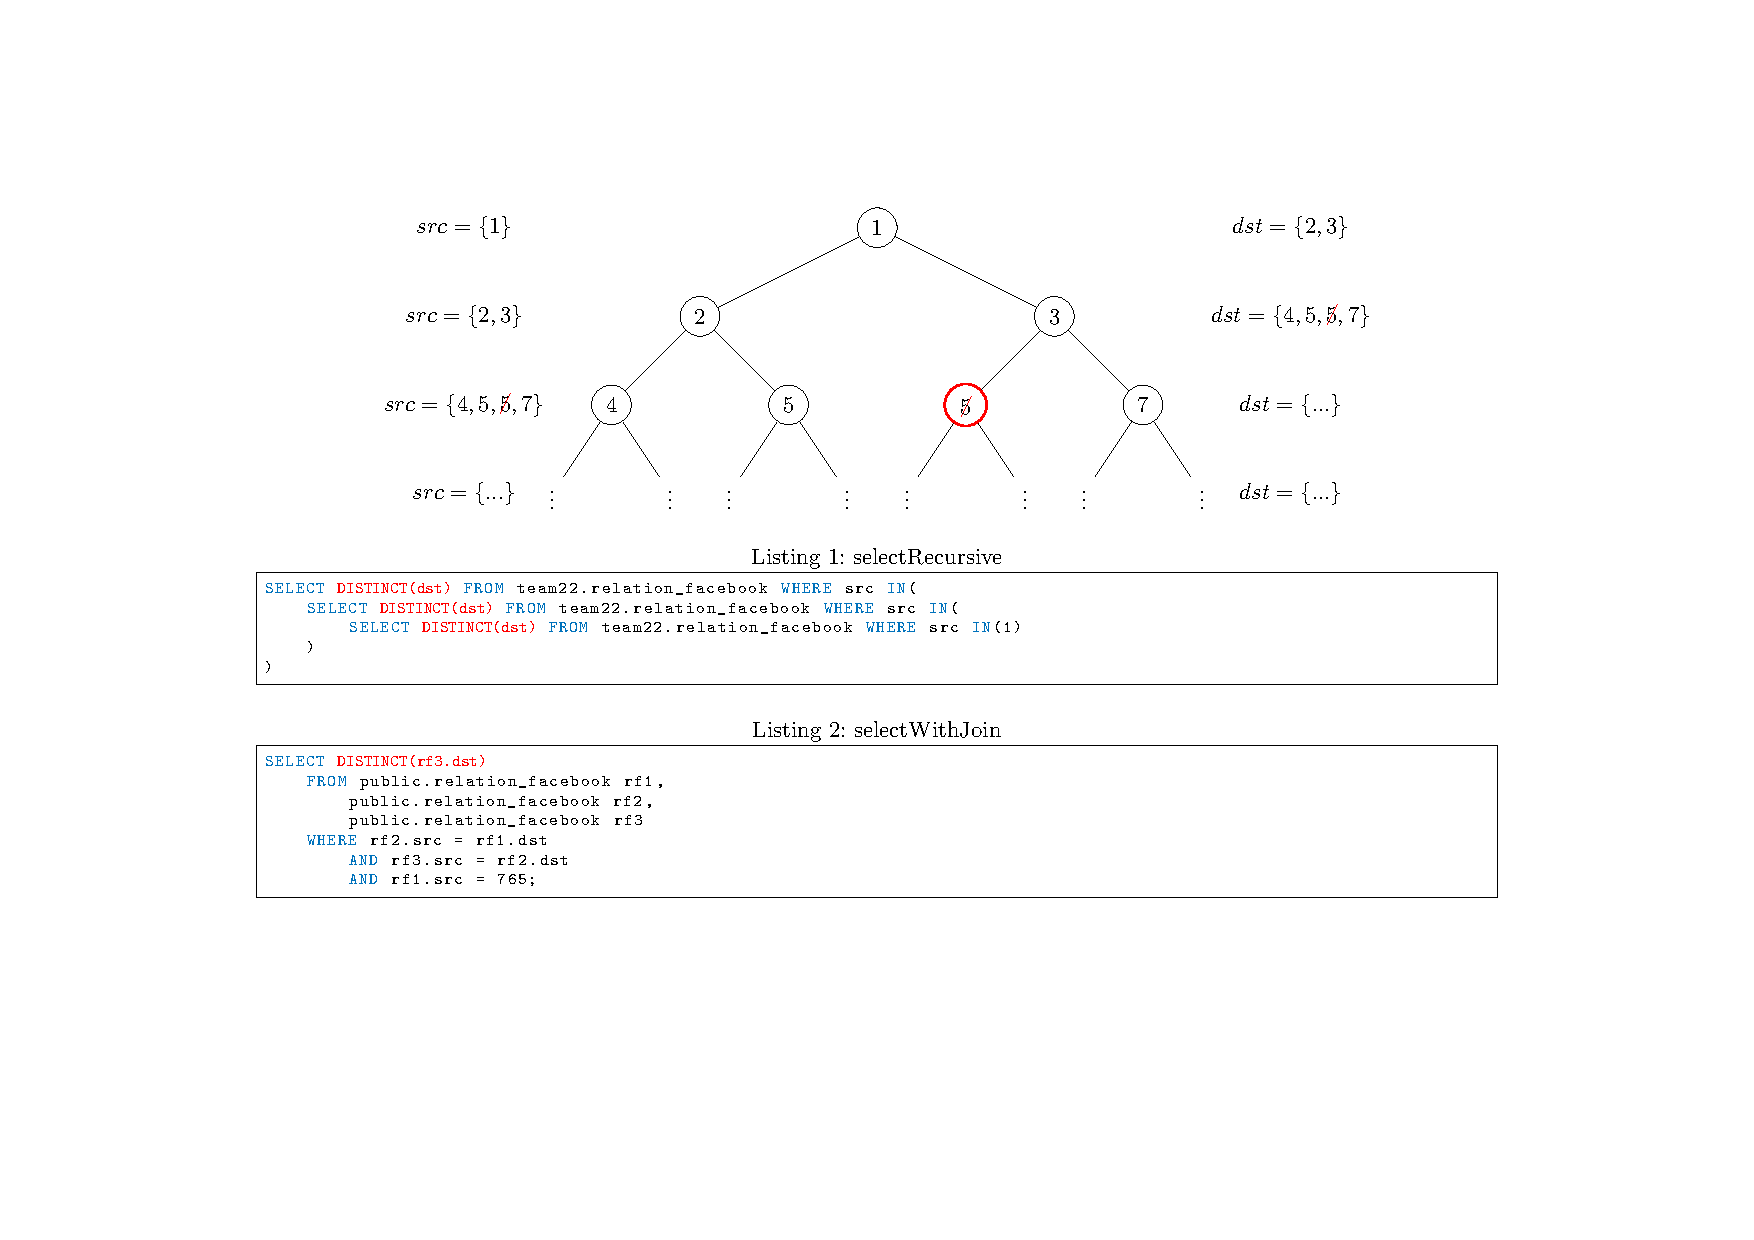
\includepdf[pages=-,fitpaper]{RecursiveSelect.pdf}
    }

%\section{PostgreSQL Überblick}

%\section{Rekursiver SQL Aufruf}
%    \begin{frame}
%        \frametitle{\rsql}
%
%    \end{frame}

\end{document}



